\chapterimage{out.png}
\chapter{Introdução - o que é programar?}

Este capítulo pretende dar apenas uma visão geral do que significa programar um computador. O leitor mais ávido por começar a experimentar pode avançar para o próximo capítulo.

\section{Programação}
``Programar'', no contexto deste manual, significa especificar um conjunto de instruções para serem executadas por uma máquina. No entanto, pode ser instrutivo fazermos a analogia máquina--pessoa para ilustrar alguns conceitos associados à programação de computadores, i.e., pensarmos em exemplos do nosso quotidiano e imaginarmo-nos a ``executar um programa''.


Considere, por exemplo, a receita do Exemplo~\ref{exe:receitaPipocas}.

\begin{lstlisting}[caption={Receita de pipocas. Adaptado de \url{http://lifestyle.sapo.pt/sabores/receitas/pipocas-doces-caseiras}.}, label=exe:receitaPipocas]
Cobre-se o fundo de um tacho com milho sem, no entanto, sobrepor. 
Rega-se o milho com um pouco de óleo e leva-se a lume brando, com o tacho tapado. 
Quando o milho começar a estalar agita-se o recipiente (sempre tapado).
Deixa-se cozinhar enquanto as pipocas estalam. 
Desliga-se, então, o lume mas só se retira a tampa quando o matraquear cessar completamente.
Agora, o adoçar: o tacho vai a lume brando, com o fundo coberto de açúcar. 
Deita-se as pipocas dentro do tacho e, quando o açúcar começar a ficar líquido, envolve-se com as pipocas utilizando para o efeito uma colher de pau. 
Movimenta-se as pipocas em sentido circular para se agarrarem ao açúcar. 
O tacho sai do lume quando o açúcar se torna amarelado.
Continua-se a mexer as pipocas até o açúcar desaparecer completamente.
\end{lstlisting}

Este primeiro exemplo serve para ilustrar algumas características da programação de computadores.%
\footnote{
Neste manual, os exemplos de código são apresentados com linhas numeradas para facilitar a referência a linhas específicas no texto. Os números propriamente ditos não fazem parte das instruções.
} %
Primeiro, a ordem das instruções é extremamente importante. A receita não funcionaria se, durante a execução, trocassemos a ordem de das instruções. Por exemplo, não faria sentido trocar as instruções das linhas 1 e 2 e regar o milho com  óleo antes de o colocar no tacho...:

\begin{lstlisting}
Rega-se o milho com um pouco de óleo e leva-se a lume brando, com o tacho tapado. 
Cobre-se o fundo de um tacho com milho sem, no entanto, sobrepor. 
. . . 
\end{lstlisting}


Segundo, as instruções são escritas na forma imperativa. A receita descreve instruções que devemos seguir para a executar convenientemente. Também ao programar podemo-nos imaginar a dar ordens a um computador.

O exemplo serve também para chamar a atenção para algumas diferenças entre a programação de um computador e a escrita de uma receita para ser seguida por uma pessoa. Se estivermos a definir um programa (receita) para ser seguido por um ser humano, as instruções que lhe damos são muito diferentes das
instruções que daríamos a um computador. O programa anterior seria facilmente executado por uma pessoa, mas não por um computador. O programa é demasiado ambíguo para ser executado por uma máquina. Por exemplo, o que significa ``um pouco de óleo''? De que forma se agita o recipiente? A linguagem natural usada no exemplo anterior serve para os seres humanos que têm naturalmente uma grande capacidade de inferir o significado das instruções pelo contexto onde são dadas. Embora com certeza todos já passamos por situações em que ficámos a pensar "o que quer dizer esta instrução?" ao seguir um manual de instruções, receita culinária, etc.

A linguagem que os computadores ``entendem'' é muito mais precisa do que a linguagem natural que usamos para comunicar entre nós. Ao programar um computador, não pode existir ambiguidade na comunicação das instruções.

%é demasiado vaga para uma máquina -- é necessário especificar qual a porta para onde devemos dirigirmo-nos. Os programas de computador necessitam, por isso, de um conjunto de instruções precisas que o computador (ou melhor, o processador do computador) saiba executar.




%Este primeiro exemplo serve para ilustrar algumas características da programação.
%Primeiro, a ordem das instruções é extremamente importante; as linhas estão numeradas para dar relevância a esse facto. O programa não funcionaria se a execução trocasse a ordem de uma das instruções para, por exemplo:
%
%\begin{lstlisting}[caption=Programa ``Atender a porta'' com instrução trocada, label=exe:atenderPortaOrdemTrocada]
%levantar da cadeira.
%dirigir-se à porta.
%abrir a porta.
%esperar que alguém bata à porta.
%perguntar em que pode ajudar.
%\end{lstlisting}
%
%Segundo, as instruções são escritas na forma imperativa. Ao programar podemo-nos imaginar a dar ordens a quem executa o programa.

%O Exemplo~\ref{exe:atenderPorta} ilustra ainda uma outra característica dos programas de computador: a entrada e saída de dados. Um programa não seria muito útil se não produzisse nada que pudesse ser utilizado pela pessoa que o executa. A saída de um programa pode tomar várias formas, e.g., números no ecrã, uma folha de papel na impressora, efeitos visuais, som, actuação física de motores de um robô, etc. Da mesma forma, a maioria dos programas permitem que o utilizador introduza, de alguma forma, dados que serão manipulados por esse programa. A forma mais típica de introdução de dados é através do rato e teclado, mas um programa pode obtê-los através de várias formas, como leitura de um ficheiro previamente escrito, leitura de sensores ligados ao computador, imagens de cameras web, áudio do microfone, etc. 



%O programa anterior seria facilmente executado por uma pessoa, mas não por um computador. O programa é demasiado ambíguo para ser executado por uma máquina. Por exemplo, o que aconteceria se a sala tivesse várias portas? Logicamente, uma pessoa iria atender a porta de onde veio o som... mas uma máquina não tem este tipo de compreensão. A instrução 
%\begin{verbatim}
%3 - dirigir-se à porta
%\end{verbatim}
%é demasiado vaga para uma máquina -- é necessário especificar qual a porta para onde devemos dirigirmo-nos. Os programas de computador necessitam, por isso, de um conjunto de instruções precisas que o computador (ou melhor, o processador do computador) saiba executar.



%\section{Algoritmos}
%Normalmente fazemos a distinção entre \emph{algoritmo} e \emph{programa}. Estes dois conceitos estão intimamente relacionados mas têm significados ligeiramente diferentes:
%\begin{description}
%\item[Algoritmos]
%Um algoritmo%
%\footnote{A palavra algoritmo tem origem no nome do matemático persa Al-Khwarizmi - 780-850.}
%é um ``conjunto de regras e operações que permitem resolver, num número finito de etapas, um problema''\cite{infopedia}.
%
%\item[Programa]
%Um programa de computador é um ``conjunto completo de instruções, em linguagem de código, que indica ao computador, passo a passo, como determinada tarefa deverá ser executada''\cite{infopedia}.
%\end{description}
%
%Dito de forma mais simples, um programa é uma implementação concreta de um algoritmo.
%
%É útil fazer esta distinção porque a definição de um algoritmo permite-nos comunicar a resolução de um problema sem nos preocuparmos com os detalhes sintácticos ou semânticos de uma determinada linguagem de programação.
%
%Normalmente os algoritmos são especificados em linguagem natural, i.e.%
%\footnote{\emph{i.e.} -- significa \emph{isto é} (do latim, \emph{id est}).}%
%, em Português, ou em pseudo-código -- uma linguagem intermédia entre a natural e uma linguagem de programação. 
%Os programas são escritos numa determinada linguagem de programação, e.g.%
%\footnote{\emph{e.g.} -- significa \emph{por exemplo} (do latim, \emph{exempli gratia}).}%
%, Processing, C, Java, ActionScript, PHP, etc.


%\section{Como Funciona o Processador de um Computador}


%\section{História Resumida das Linguagens de Programação}


\section{Linguagens de Programação}
Existem várias linguagens que podemos utilizar para programar um computador. Algumas apenas funcionam em determinados ambientes, por exemplo, o ActionScript é uma linguagem para programar Flash, ou seja apenas funciona no programa Macromedia Flash.
O PHP, por outro lado, serve apenas para programar servidores de páginas web, i.e., não podemos criar um programa de desktop com janelas e botões em PHP.
A linguagem C, por outro lado é uma linguagem mais tradicional e universal -- serve para escrever programas que correm directamente num computador de desktop, assim como programas que correm em servidores.

Apenas como curiosidade, aqui fica uma pequena lista das linguagens de programação mais comuns:
\begin{description}

\item[C e C++] são duas linguagens. C++ é uma evolução da linguagem C, que por sua vez é uma das linguagens mais utilizadas e mais antigas. A linguagem C foi originalmente criada por Dennis Ritchie entre 1969 e 1973 e foi usada para implementar um dos sistemas operativos mais poderosos: o Unix. O exemplo seguinte mostra um programa básico escrito em C%
\footnote{
Um programa pequeno como este designa-se usualmente por ``Hello World'' por ilustrar a estrutura e funcionalidade mais básicas de uma linguagem.
}%
.
\begin{lstlisting}
#include <stdio.h>
 
int main(void)
{
    printf("hello, World\n");
}
\end{lstlisting}
Quando executado, este programa apenas escreve no ecrã do computador o texto ``Hello, World''. (Na verdade o texto é escrito naquilo que se chama a consola e que representa uma área para saída de texto apenas.)

\item[Java] é uma linguagem de programação criada em 1995 pela empresa Sun Microsystems com o objectivo de permitir a criação de programas que pudessem ser executados em várias plataformas. A sua utilização tornou-se mais conhecida através das \emph{applets} -- pequenos programas que podem ser executados num browser. Neste momento é uma linguagem genérica utilizada tanto para criar aplicações de computadores de secretária como para programar servidores.
O exemplo seguinte ilustra um programa mínimo em Java:
\begin{lstlisting}
public class HelloWorld {
	public static void main(String[] args) {
		System.out.println("Hello, World");
    }
}
\end{lstlisting}
Tal como o exemplo em C, este exemplo apenas escreve o texto ``Hello, World'' na consola do computador.

\item[Processing] é uma linguagem de programação baseada na linguagem Java. Foi criada para simplificar a programação em Java e para servir como ferramenta de programação orientada para artistas digitais e para o ensino da programação. O exemplo seguinte tem o mesmo efeito que o exemplo anterior em Java, mas como se pode ver é bem mais simples:
\begin{lstlisting}
println("Hello, World");
\end{lstlisting}

No entanto, Processing é uma linguagem muito direccionada para a geração de imagens pelo que o exemplo seguinte é mais ilustrativo de um programa nesta linguagem:
\begin{lstlisting}
void setup() {
	size(400, 400);
}
 
void draw() {
	line(150, 25, mouseX, mouseY);
}
\end{lstlisting}
Este exemplo cria uma pequena janela gráfica de 400 por 400 pixeis e desenha uma linha entre os pontos (150, 25) e a posição do cursor do rato. Este exemplo é interactivo: podemos mover o rato sobre a janela e o programa actualiza automaticamente o desenho da linha. 

\item[PHP] é uma linguagem de programação diferente das anteriores porque é direccionada apenas para servidores Web. Esta linguagem não permite criar um programas para serem executado num computador pessoal (com janelas, menus, botões, etc.). É destinada à criação de páginas Web e, por isso, executa não no nosso computador, mas nos servidores que alojam as páginas. O exemplo seguinte mostra um exemplo de PHP embutido numa página Web (o código PHP é apenas a linha \ref{php:line}, o resto é HTML -- a linguagem para descrever páginas Web.).
\begin{lstlisting}[escapechar=|]
<html>
	<head>  
		<title>PHP Test</title>
	</head>
	<body>
		<?php echo '<p>Hello World</p>'; ?> |\label{php:line}|
	</body>
</html>
\end{lstlisting}

\end{description}

\subsection{Compilar e Executar}
Internamente, um computador trabalha apenas com números. Toda a informação com que trabalhamos quando usamos um computador é representada pelo computador através de números. Um programa de computador é também ele representado por números. 

Nos primeiros computadores, a programação era feita usando instruções entendidas directamente pelo computador (números). Estas instruções são designadas por código máquina. 
%Computadores diferentes (com processadores diferentes) possuem conjuntos de instruções diferentes, pelo que um programa escrito em código máquina apenas executa num determinado tipo de computador. 
A programação em código máquina era muito trabalhosa e propícia a erros, pelo que foram criadas linguagens de programação  mais próximas da nossa linguagem natural. No entanto, a introdução destas linguagens obriga a uma conversão entre o código escrito pelo programador, o chamado código fonte, e o código máquina. O processo de conversão chama-se compilação (ver Figura~\ref{fig:processo-compilacao}). 

\begin{figure}[!ht]
	\centering
		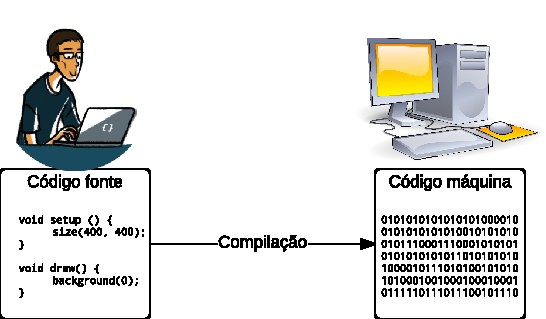
\includegraphics[width=8cm]{images/DiagramaCompilacao.pdf}
	\caption{Processo de compilação.}
	\label{fig:processo-compilacao}
\end{figure}

O processo de compilação consiste em analisar o código fonte para verificar se está de acordo com as regras gramaticais da linguagem que se está a usar e em converter esse código fonte em código máquina. A ferramenta que se usa para compilar é ela própria um programa de computador -- o compilador. 

O resultado da compilação é um ficheiro (ou conjunto de ficheiros) que podem ser executados.

Neste manual, o compilador é algo que está ``escondido'' e com o qual não temos de nos preocupar na maioria das situações. No próximo capítulo, veremos na prática como escrever e executar os nossos programas.

%
%\section{Lógica e Sintaxe}
%O código fonte de um programa pode ser visto de duas perspectivas: da lógica do programa; e da sintaxe.
%
%Uma determinada linguagem de programação é definida principalmente pela sua sintaxe, ou seja pelas regras que definem o que é um programa bem escrito. Da mesma forma que a sintaxe da língua Portuguesa define as regras de construção de frases, também a sintaxe da linguagem de programação define as regras de construção de um programa escrito nessa linguagem. Por exemplo, a frase ``O João foi às compras.'', está de acordo com as regras, mas ``O João às foi compras.'', não está. Apesar de o significado de ambas as frases ser óbvio e idêntico: o João foi às compras, a segunda quebra as regras da construção de frases em Português.
%
%A lógica de um programa equivale ao seu significado. No exemplo anterior a lógica (significado) da frase era óbvia, mas estava mal construida. Também um programa pode estar logicamente correcto, mas sintacticamente incorrecto. Um programa sintacticamente incorrecto não pode ser compilado (os compiladores não são ``suficientemente inteligentes'' para perceberem o significado do programa de modo a corrigirem a sintaxe). Os erros sintácticos são facilmente detectados pelo compilador.
%De forma inversa, um programa pode estar sintacticamente correcto, mas logicamente não. Nestes casos, o programa é compilado e executado, mas o resultado não é o que o programador estava à espera. Estes erros são mais difíceis de detectar!
%
%
%
%
%\section{Nível de Detalhe}
%Quando escrevemos um programa em Português a que nível de detalhe devemos ir na especificação das instruções?
%Por exemplo, se quisermos escrever um programa para uma pessoa mudar um pneu de um carro podemos ter algo como o seguinte:
%\begin{verbatim}
%1 - sair do carro.
%2 - abrir a mala do carro.
%3 - tirar pneu sobresselente.
%4 - tirar macaco.
%5 - tirar chave.
%6 - desapertar ligeiramente as porcas do pneu.
%7 - colocar o macaco debaixo do carro.
%8 - dar \'a manivela até o pneu ficar suficientemente levantado.
%9 - desapertar as porcas na totalidade.
%10 - retirar o pneu furado.
%11 - colocar o pneu novo.
%12 - apertar as porcas.
%13 - baixar o carro.
%14 - retirar o macaco.
%15 - apertar bem as porcas.
%16 - guardar chave.
%17 - guardar macaco.
%18 - guardar pneu furado.
%\end{verbatim}
%
%Mas, estamos a assumir que a pessoa sabe fazer uma série de coisas, como sair do carro, abrir a mala, etc.
%Cada um dos passos do nosso programa anterior pode ele mesmo ser um programa em si. Por exemplo sair do carro:
%\begin{verbatim}
%1 - desligar o carro.
%2 - apertar o travão de mão.
%3 - retirar o cinto de segurança.
%4 - retirar a chave da ignição.
%5 - abrir a porta.
%6 - sair.
%7 - fechar a porta.
%\end{verbatim}
%
%Então, a que nível de detalhe deveremo ir quando estamos a escrever um programa? No caso de um programa para ser executado por uma pessoa, devemos descer ao nível de detalhe suficiente para a pessoa conseguir executar cada passo. Obviamente, isto depende da tarefa e da pessoa.
%
%No caso de um programa de computador, o problema não se coloca a este nível. Ao utilizarmos uma determinada linguagem de programação, estamos automaticamente limitados às instruções mais básicas fornecidas por essa linguagem. Por exemplo, no caso do desenho num ecrã, algumas linguagens apenas possuem instruções para desenhar um pixel numa determinada posição do ecrã. Neste caso, se quisermos fazer uma programa para desenhar uma linha vertical teriamos de fazer algo do género:
%\begin{verbatim}
%1 - desenhar pixel na primeira posicao da linha.
%2 - avancar um pixel na vertical.
%3 - desenhar um pixel na nova posicao.
%4 - repetir o passo 2 até chegar ao final da linha.
%\end{verbatim}
%
%Outras linguagens têm instruções para desenhar linhas, pelo que o programa anterior se resumiria a uma única instrução:
%\begin{verbatim}
%1 - desenhar linha vertical.
%\end{verbatim}
%
%Ou seja, quando programamos um computador temos de utilizar as instruções fornecidas pela linguagem que estamos a utilizar. Daí que algumas linguagens sejam mais aplicadas nalguns tipos de programas -- possuem instruções que facilitam a escrita de determinados programas.
%
%No entanto, o problema do nível de detalhe coloca-se sob outra perpectiva quando programamos um computador. Todas as linguagens permitem-nos definir as nossas próprias instruções compostas por sequências maiores de instruções básicas. Por exemplo, no caso da linguagem que apenas permite desenhar um pixel numa posição do ecrã, poderiamos compor uma nova instrução: \texttt{desenharLinhaVertical}, à custa dos passos do nosso programa exemplo. Assim, sempre que quisessemos desenhar uma linha vertical no ecrã bastava usar a nova instrução:
%\begin{verbatim}
%1 - desenharLinhaVertical.
%\end{verbatim}
%
%Quando escrevemos um programa devemos pensar em agrupar conjuntos de instruções de forma a termos ao nosso dispor instruções que efectuam vários passos de cada vez. 
%A questão agora é saber que instruções agrupar. Novamente, não há uma resposta única. Depende do programa. É uma questão de experiência (e, às vezes, de estilo do programador).

\section{Conceitos Básicos de Um Programa}
Quando criamos programas, ou, de forma mais genérica, quando pensamos em algoritmos, existem alguns conceitos fundamentais que são comuns a todos eles: \emph{memória}, \emph{selecção}, \emph{iteração} e \emph{abstracção}.

\begin{description} \itemsep5pt %\parskip0pt \parsep0pt
\item[Memória]O conceito de memória será aprofundado no Capítulo~\ref{cap:memoria}.
A memória é o que permite ao nosso programa guardar dados temporários ou intermédios para serem utilizados mais tarde.
Por exemplo, se pretendêssemos criar um programa para calcular os pontos de uma equipa no campeonato de futebol faríamos algo do género\footnote{
Este exemplo está escrito em pseudo-código -- uma linguagem sem uma sintaxe formalmente definida, mas em que o significado das instruções é mais ou menos óbvio. O pseudo-código é bom para explicar um algoritmo a outra pessoa, mas não é compilável para correr num computador.
}%
:
\begin{lstlisting}
ler jogosGanhos.
ler jogosEmpatados.
pontos = jogosGanhos * 3 + jogosEmpatados * 1.
escrever pontos.
\end{lstlisting}
No programa anterior a instrução \texttt{ler}, coloca numa \emph{variável} um valor fornecido pelo utilizador. Uma variável
é a memória do nosso programa. É como uma gaveta com nome, na qual podemos guardar valores para mais tarde utilizar.
O programa anterior precisa de guardar os valores do número de jogos ganhos e empatados para poder efectuar a operação matemática que devolve o número de pontos no campeonato. O resultado desse cálculo, é, ele mesmo, colocado também numa ``gaveta'' para posterior utilização. Uma vez colocados na ``gaveta'', os dados podem ser consultados em qualquer altura (ponto de execução) do nosso programa. 


\item[Selecção] O conceito de selecção será aprofundado no Capítulo~\ref{cap:seleccao}.
O conceito de \emph{selecção} está associado ao caminho executado pelo nosso programa. Um programa pode ser visto como uma árvore: a execução começa por um ponto comum -- o tronco, e, à medida que o programa executa, pode percorrer um ramo ou outro, dependendo das circunstâncias no momento da execução.
Por exemplo, no programa seguinte:
\begin{lstlisting}
ler jogosGanhosFCP.
ler jogosEmpatadosFCP.
ler jogosGanhosSLB.
ler jogosEmpatadosSLB.
pontosFCP = jogosGanhosFCP * 3 + jogosEmpatadosFCP.
pontosSLB = jogosGanhosSLB * 3 + jogosEmpatadosSLB.
se pontosFCP > pontosSLB então 
	escrever "O FCP está à frente do SLB".
senão
	escrever "O SLB está à frente do FCP".     
\end{lstlisting}

existe um ``tronco'' comum a todas as execuções do programa -- as linhas de 1 a 7.
No entanto, consoante a pontuação de uma e outra equipa, o programa pode percorrer o ramo 8 -- se o FCP tiver mais pontos que o SLB, ou o ramo 10 -- se o SLB tiver mais pontos que o FCP.
A linha\footnote{O símbolo ``>'' significa ``maior do que''.}: 
\begin{lstlisting}[firstnumber=7]
se pontosFCP > pontosSLB então      
\end{lstlisting}

\emph{selecciona} o ramo a executar no programa.%
\footnote{As linhas 8 e 10 estão \emph{indentadas}, isto é, escritas mais à direita, para facilitar a leitura do programa. Desta forma é óbvio que o ramo 8 corresponde à condição ser verdadeira e o 10 à condição falsa. Caso contrário, não seria facilmente perceptível que o programa contém ramos.}

\item[Iteração] O conceito de iteracção será aprofundado no Capítulo~\ref{cap:iteraccao}.
A maior parte dos programas que escrevemos contêm partes que são repetidas várias vezes. Por exemplo, se quisermos calcular as pontuações de todas as equipas do campeonato, poderíamos construir um programa do género:

\begin{lstlisting}
ler jogosGanhosEquipa1.
ler jogosEmpatadosEquipa1.
pontosEquipa1 = jogosGanhosEquipa1 * 3 + jogosEmpatadosEquipa1.
escrever pontosEquipa1.
ler jogosGanhosEquipa2.
ler jogosEmpatadosEquipa2.
pontosEquipa2 = jogosGanhosEquipa2 * 3 + jogosEmpatadosEquipa2.
escrever pontosEquipa2.
ler jogosGanhosEquipa3.
ler jogosEmpatadosEquipa3.
pontosEquipa3 = jogosGanhosEquipa3 * 3 + jogosEmpatadosEquipa3.
escrever pontosEquipa3.
...
ler jogosGanhosEquipa18.
ler jogosEmpatadosEquipa18.
pontosEquipa18 = jogosGanhosEquipa18 * 3 + jogosEmpatadosEquipa18.
escrever pontosEquipa18.
\end{lstlisting}
Neste programa, para calcular a pontuação de 18 equipas, precisamos de 72 linhas de código! No entanto, se olharmos bem, as linhas são muito parecidas -- as primeiras 4 linhas repetem-se ao longo do programa. Existe uma estrutura que nos permite economizar linhas de código: o \emph{ciclo}:

\begin{lstlisting}
i = 1.
enquanto i <= 18 fazer:
	ler jogosGanhosEquipa.
    ler jogosEmpatadosEquipa.
    pontosEquipa = jogosGanhosEquipa * 3 + jogosEmpatadosEquipa.
    escrever pontosEquipa.
    i = i + 1.
\end{lstlisting}
Neste caso, colocamos as 4 linhas repetidas do programa anterior dentro daquilo a que chamamos \emph{ciclo} -- uma estrutura que itera a execução das linhas de código%
\footnote{Não confundir \emph{iterativo} -- que se repete; com \emph{interactivo} -- que permite a troca de informação entre sistema e utilizador.}%
. 
Basicamente, o programa utiliza uma variável para contar as equipas que já calculámos: a variável \texttt{i}.

\item[Abstracção] O conceito de iteracção será aprofundado no Capítulo~\ref{cap:funcoes}. A abstracção permite-nos criar programas altamente complexos, dividindo-os em componentes mais simples. Por exemplo, vamos supor que queríamos calcular a soma de dois factoriais%
\footnote{O factorial de um número é o produto de todos os números inteiros positivos menores ou iguais a esse número.}:
\begin{lstlisting} 
ler numero1.
i = 1.
factorial1 = 1.
enquanto i <= numero1 fazer:
	factorial1 = factorial1*i.
	i = i + 1.

ler numero2.
i = 1
factorial2 = 1.
enquanto i <= numero2 fazer:
	factorial2 = factorial2*i.
	i = i + 1.

soma =  factorial1 + factorial2.
escrever soma.
\end{lstlisting}
A leitura deste programa pode ser simplificada se criarmos uma \emph{função} para calcular o factorial:
\begin{lstlisting} 
ler numero1.
factorial1 = calculaFactorial(numero1).

ler numero2.
factorial2 = calculaFactorial(numero2).

soma =  factorial1 + factorial2.
escrever soma.


função calculaFactorial(numero) 
	i = 1.
	factorial = 1.
	enquanto i <= numero fazer:
		factorial = factorial*i.
		i = i + 1.
	devolve factorial

\end{lstlisting}
O programa principal torna-se assim mais fácil de ler e de entender que calcula a soma de dois factoriais. A função é uma estrutura que nos permite não só abstrair da complexidade da implementação do cálculo do factorial, como reutilizar o código que faz esse cálculo.
\end{description}



\section{Exercícios Resolvidos}

\begin{enumerate}
	\item \label{exe:1_1} Escreva um programa em linguagem natural para ligar os computadores de uma sala de aulas. Escreva o programa para ser seguido por uma pessoa. O programa deve ter pelo menos uma tomada de decisão.
	
	\item \label{exe:1_2} Baseando-se no programa que escreveu no ponto anterior, substitua cada instrução desse programa por um conjunto de instruções mais detalhadas.
	
	\item \label{exe:1_3} Baseando-se no programa que escreveu no ponto anterior, tente agrupar conjuntos de instruções em funções, de forma a tornar o programa mais fácil de ler.
\end{enumerate}



\section{Exercícios para Resolver}
\begin{enumerate}
\item 
Pensar num programa que possa ser facilmente implementado por um colega seu na sala de aula. Escrever esse programa.  O programa deve ter mais de 10 instruções, deve ter pelo menos uma estrutura de selecção ou iteração e deve poder ser executado em menos de 5 minutos.

\item Escreva o programa anterior com um nível de detalhe maior.

\item Agrupar algumas instruções do programa anterior em funções de forma a tornar o programa mais legível.
\end{enumerate}



\clearpage
\section{Resolução dos Exercícios Resolvidos}


\subsubsection*{Exercício Resolvido \ref{exe:1_1}}
\begin{lstlisting}
//Programa Ligar os Computadores da Sala

Dirigir-se ao primeiro computador.
Carregar no botão de ``power'' do computador.
Carregar no botão de ``power'' do monitor.
Se computador não ligou
	Verificar cabos de alimentação
	Repetir o passo 3.
Verificar se há mais computadores     
Se houver mais computadores então
	Dirigir-se ao computador seguinte.
	Repetir o passo 3.
Senão
	Termina.    
\end{lstlisting}
\paragraph{Notas}
Este programa funciona apenas se determinadas condições se verificarem. Uma vez que 
não colocámos instruções para verificar se o computador já estava ligado, caso
isso aconteça o computador será desligado. Para o programa funcionar como
pretendido é necessário que todos estejam desligados.


\subsubsection*{Exercício \ref{exe:1_2}}

\begin{lstlisting}
//Programa Ligar os Computadores da Sala (mais detalhe)

Dirigir-se ao primeiro computador.
Verificar se o computador está desligado.
Se o computador estiver desligado então
	Identificar botão de ``power'' do computador.
	Levantar a mão e esticar o dedo indicador.
	Pressionar o botão de ``power'' do computador.
Verificar se o monitor está desligado.
Se o monitor estiver desligado então
	Identificar botão de ``power'' do monitor.
	Levantar a mão e esticar o dedo indicador.
	Pressionar o botão de ``power'' do monitor.
Se computador não ligou
	Verificar cabos de alimentação do computador.
	Verificar os cabos de alimentação do monitor.
	Repetir o passo 5.
Verificar se há mais computadores     
Se houver mais computadores então
	Dirigir-se ao computador seguinte.
	Repetir o passo 24.
Senão
	Termina.    
\end{lstlisting}

\subsubsection*{Exercício \ref{exe:1_3}}
\begin{lstlisting}
//Programa Ligar os Computadores da Sala (mais detalhe)

Dirigir-se ao primeiro computador.
Ligar o Computador
Ligar o Monitor
Se computador não ligou
	Verificar cabos de alimentação do computador.
	Verificar os cabos de alimentação do monitor.
	Repetir o passo 4.
Verificar se há mais computadores     
Se houver mais computadores então
	Dirigir-se ao computador seguinte.
	Repetir o passo 4.
Senão
	Termina.
    
    
Função Ligar o Computador:
	Verificar se o computador está desligado.
	Se o computador estiver desligado então
		Identificar botão de ``power'' do computador.
		Levantar a mão e esticar o dedo indicador.
		Pressionar o botão de ``power'' do computador.


Função Ligar o Monitor:
	Verificar se o monitor está desligado.
	Se o monitor estiver desligado então
		Identificar botão de ``power'' do monitor.
		Levantar a mão e esticar o dedo indicador.
		Pressionar o botão de ``power'' do monitor.
\end{lstlisting}
